\section{Durchführung}
\subsection{Versuchsaufbau}
Der genutzte Versuchsaufbau ist in Abb.\ref{Aufbau} dargestellt. Die Lichtquelle des Aufbaus ist eine Halogen-Lampe, welche ein Spektrum hat das größtenteils im Infrarot bereich liegt. Das emittierte Licht wird durch eine Linse gebündelt und durch einen Lichtzerhacker in Pulse eingeteilt.
Die Lineapolarisierung des Lichts erfolgt durch ein Glan-Thompson-Prisma, dessen Winkel zum Strahl durch ein Goniometer variiert werden kann. Die Photonen treffen danach auf die scheibenförmige Probe, welche in einem Elektromagneten mit Feldrichtung parallel zur Photonenrichtung platziert ist. Hinter der Probe befindet sich eine Halterung für austauschbare Interferenzfilter. Zur Untersuchung der Rotation der Polarisationsebene wird die Strahlung mit einem zweiten Glan-Thompson-Prisma in zwei senkrecht zueinander polarisierte Teile  zerlegt und die Teilstrahle werden erneut durch Linsen gebündelt und die Lichtintensität wird mitel Photowiderständen gemessen. Die hohe Rauschspannung welche an den Photowiderständen auftritt wird durch die Wechsellichtmethode, welche durch den Lichtzerhacker und einen auf die Frequenz des Zerhackers eingestellten Selektivverstärker gegeben ist, verhindert. Die am Photowiderstand wird an Kondensatoren ausgegekopplet, wobei die Zeitkonstante von einem der Kondensatoren variabel ist. Die Signale beider Photowiderstände werden aufeinen Differenzverstärker gegeben und von dort in den Selektivverstärker. Das Signal des Selektivverstärkers wird an einem Oszilloskop angezeigt.
\begin{figure}[H]
  \centering
  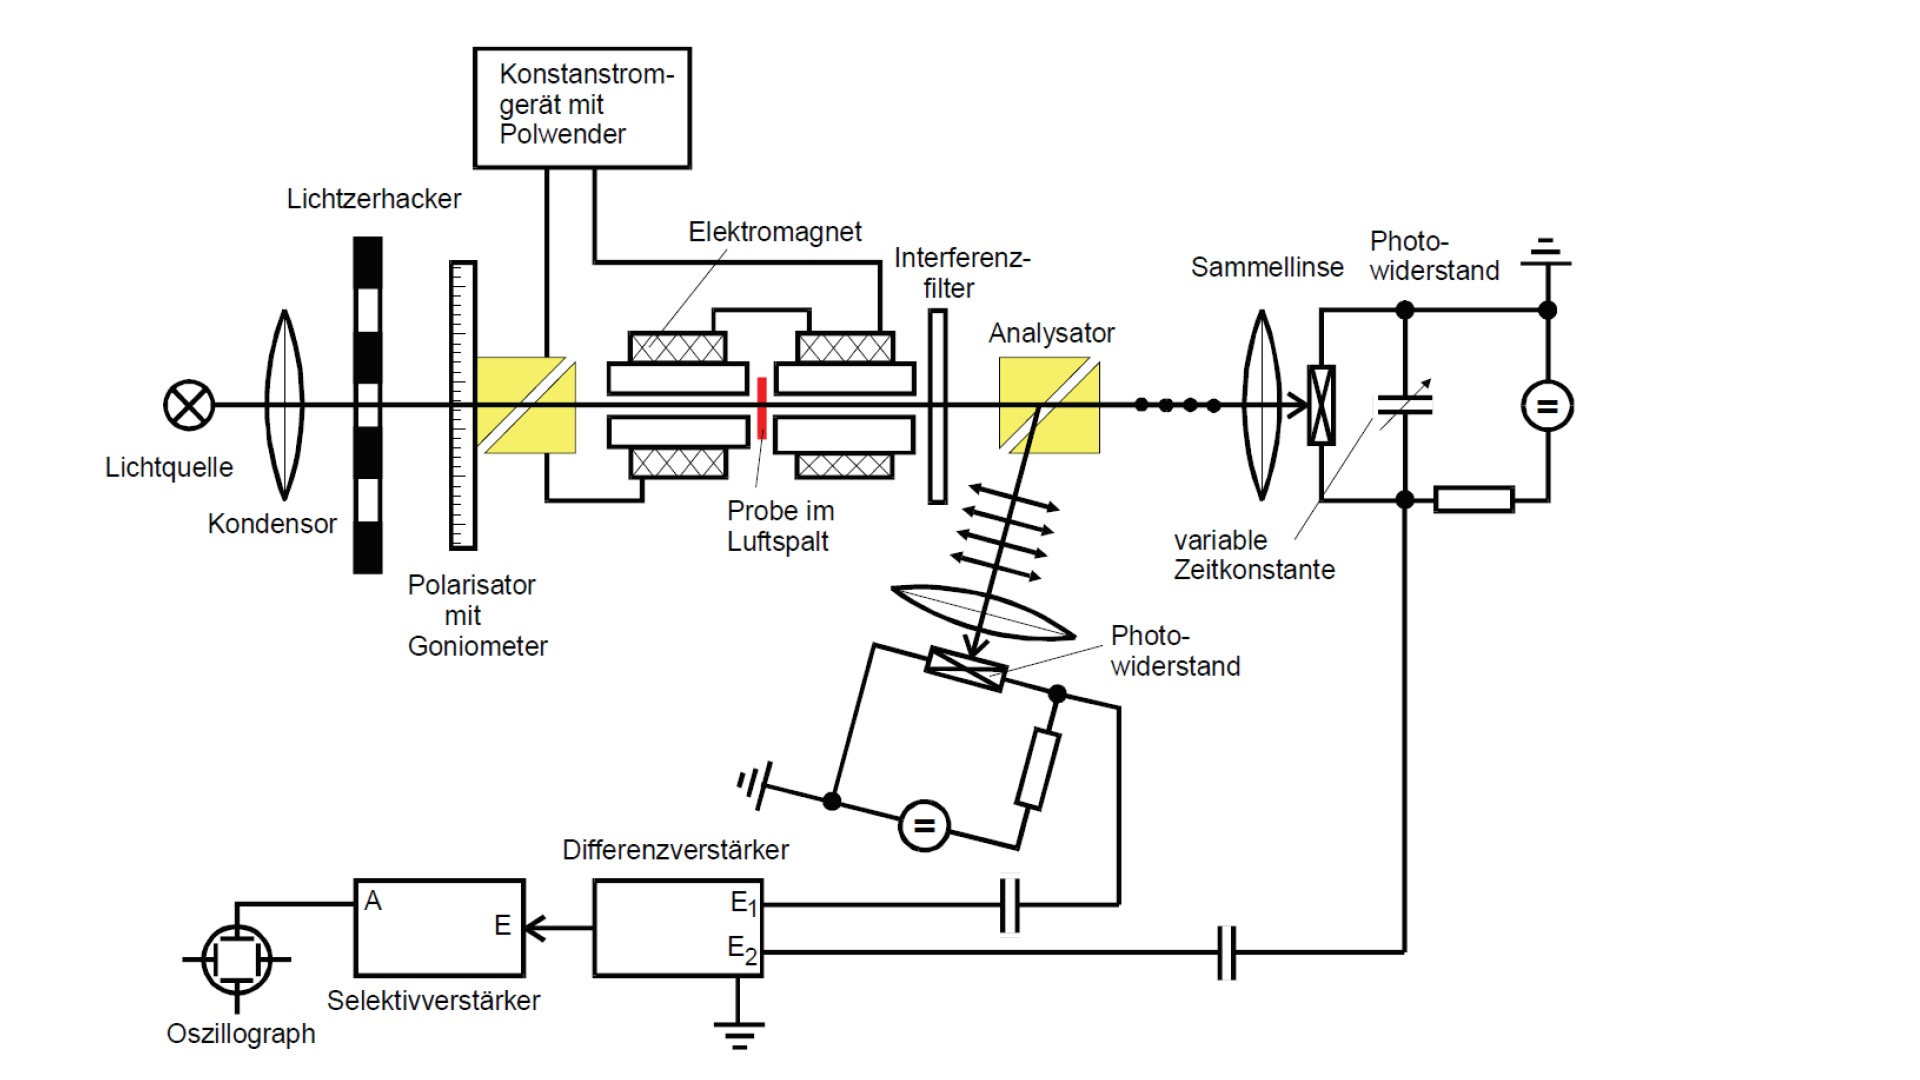
\includegraphics[width=1\textwidth]{bilder/aufbau.png}
  \caption{Schematische Darstellung des genutzten Versuchsaufbaus \cite{anleitung}.}
  \label{Aufbau}
\end{figure}
\subsection{Versuchsdurchführung}
\subsubsection{Justierung}
Zu Beginn des Versuchs muss der Aufbau justiert werden. Hierzu werden Probe, Interferenzfilter und die Abdeckungen der Photowiderstandgehäuse entfernt. Der Strahlenganz des Lichts wird überprüft und es wird getestet ob die Veränderungen am Goniometer die erwarteten Intensitätschwankungen an den Teilstrahlen verursachen.\\
Anschließend kann der Lichtzerhacker eingeschaltet und auf eine Frequenz von $450\si{\Hz}$ gestellt werden. Die Mittenfrequenz des Selektivverstärkers wird auf auf den Zerhacker angepasst indem man das Signal eines Photowiderstands am Differenzverstärker gegen ein "Ground"-Signal schaltet und das resultierende Signal in den Selektivverstärker gibt. Die Frequenz des Selektivverstärkers wird solange variiert bis man ein maximales Signal bekommt.
\subsubsection{Messung}
Zur Bestimmung des Drehwinkels wird eine Probe und ein Interferenzfilter in den Aufbau eingesetzt und es wird der Elektromagnet auf die maximale Leistung eingestellt. Mittels des Goniometers wird die Intensität der Teilstrahlen so eingestellt, dass das Signal am Oszilloskop Null wird. Ist dies erreicht so wird der am Goniometer eingestellte Winkel aufgezeichnet und das B-Feld wird umgepolt. Nun werden erneut die beiden Teilstrahlen abgeglichen und der eingestellte Winkel aufgezeichnet. Die Messung wird für Drei Proben und Neun Interferenzfilter durchgeführt. Abschließen wird noch die Stärke des B-Feldes mit einer Halls-Sonde bestimmt. 
